%----------------------------------------------------------------------------------------
%	PACKAGES AND THEMES
%----------------------------------------------------------------------------------------

\documentclass{beamer}

\mode<presentation> {

% The Beamer class comes with a number of default slide themes
% which change the colors and layouts of slides. Below this is a list
% of all the themes, uncomment each in turn to see what they look like.

%\usetheme{default}
\usetheme{AnnArbor}
%\usetheme{Antibes}
%\usetheme{Bergen}
%\usetheme{Berkeley}
%\usetheme{Berlin}
%\usetheme{Boadilla}
%\usetheme{CambridgeUS}
%\usetheme{Copenhagen}
%\usetheme{Darmstadt}
%\usetheme{Dresden}
%\usetheme{Frankfurt}
%\usetheme{Goettingen}
%\usetheme{Hannover}
%\usetheme{Ilmenau}
%\usetheme{JuanLesPins}
%\usetheme{Luebeck}
%\usetheme{Madrid}
%\usetheme{Malmoe}
%\usetheme{Marburg}
%\usetheme{Montpellier}
%\usetheme{PaloAlto}
%\usetheme{Pittsburgh}
%\usetheme{Rochester}
%\usetheme{Singapore}
%\usetheme{Szeged}
%\usetheme{Warsaw}

% As well as themes, the Beamer class has a number of color themes
% for any slide theme. Uncomment each of these in turn to see how it
% changes the colors of your current slide theme.

%\usecolortheme{albatross}
%\usecolortheme{beaver}
%\usecolortheme{beetle}
%\usecolortheme{crane}
%\usecolortheme{dolphin}
%\usecolortheme{dove}
%\usecolortheme{fly}
%\usecolortheme{lily}
%\usecolortheme{orchid}
%\usecolortheme{rose}
%\usecolortheme{seagull}
%\usecolortheme{seahorse}
%\usecolortheme{whale}
%\usecolortheme{wolverine}

%setbeamertemplate{footline} % To remove the footer line in all slides uncomment this line
%\setbeamertemplate{footline}[page number] % To replace the footer line in all slides with a simple slide count uncomment this line

\setbeamertemplate{navigation symbols}{} % To remove the navigation symbols from the bottom of all slides uncomment this line
}
\usepackage{tikz}
\usepackage{ifthen}
\usepackage{graphicx} % Allows including images
\usepackage{booktabs} % Allows the use of \toprule, \midrule and \bottomrule in tables
\usepackage{amsmath}

%----------------------------------------------------------------------------------------
%	TITLE PAGE
%----------------------------------------------------------------------------------------

\title[2016 winter school]{Estimation and Accuracy after Model Selection} % The short title appears at the bottom of every slide, the full title is only on the title page

\author[Yongchan Kwon]{Yongchan Kwon} % Your name
\institute[] % Your institution as it will appear on the bottom of every slide, may be shorthand to save space
{
\textit{Department of Statistics, Seoul National University, Seoul,  Korea}
}
\date{February 26, 2016}

\begin{document}

\begin{frame}
\titlepage % Print the title page as the first slide
\end{frame}

\begin{frame}
\frametitle{Contents} % Table of contents slide, comment this block out to remove it
\tableofcontents % Throughout your presentation, if you choose to use \section{} and \subsection{} commands, these will automatically be printed on this slide as an overview of your presentation
\end{frame}

%----------------------------------------------------------------------------------------
%	PRESENTATION SLIDES
%----------------------------------------------------------------------------------------

%------------------------------------------------
% Sections can be created in order to organize your presentation into discrete blocks, all sections and subsections are automatically printed in the table of contents as an overview of the talk
\section{Introduction}
%------------------------------------------------
%\subsection{Subsection Example} % A subsection can be created just before a set of slides with a common theme to further break down your presentation into chunks
\begin{frame}
\frametitle{Motivating example}
\begin{itemize}
\item $n=164$ men took Cholestyramine for $\sim$ 7 years
\item $x=$ compliance measure (normalized)
\item $y=$ cholesterol decrease
\item Regression $y$ on $x$ ? Wish to estimate $\mu_j = E[y_j \mid x_j]$ for $j=1,\dots,n$
\end{itemize}
\end{frame}
%------------------------------------------------
\begin{frame}
\frametitle{Motivating example}
\begin{figure}[h]
\centering
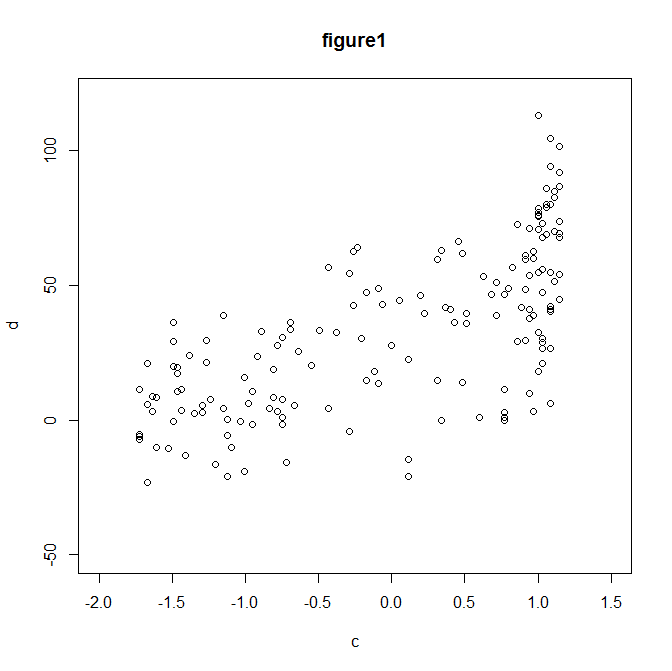
\includegraphics[width=200bp, height= 180bp]{figure1-1.png}
\caption{Cholesterol data, n=164 subjects: cholesterol decrease plotted versus normalized compliance}
\end{figure}
\end{frame}
%------------------------------------------------
\begin{frame}
\frametitle{Motivating example}
\begin{itemize}
\item Regression Model: $y= X\beta + e$, $[e_i \sim (0, \sigma^2)]$
\item $C_p$ Criterion: $\| y-X\hat{\beta}\|^2 + 2m\sigma^2$\\
$\hat{\beta}=$OLS estimate, $m=$''degree of freedom''
\item Model Selection: from possible models $M_1, M_2, M_3, \dots,$ choose the one minimizing $C_p$.
\item Then use OLS estimate from chosen model. (Assume model selection procedure is known)
\end{itemize}
\end{frame}
%------------------------------------------------
\begin{frame}
\frametitle{Motivating example}
\begin{figure}[h]
\centering
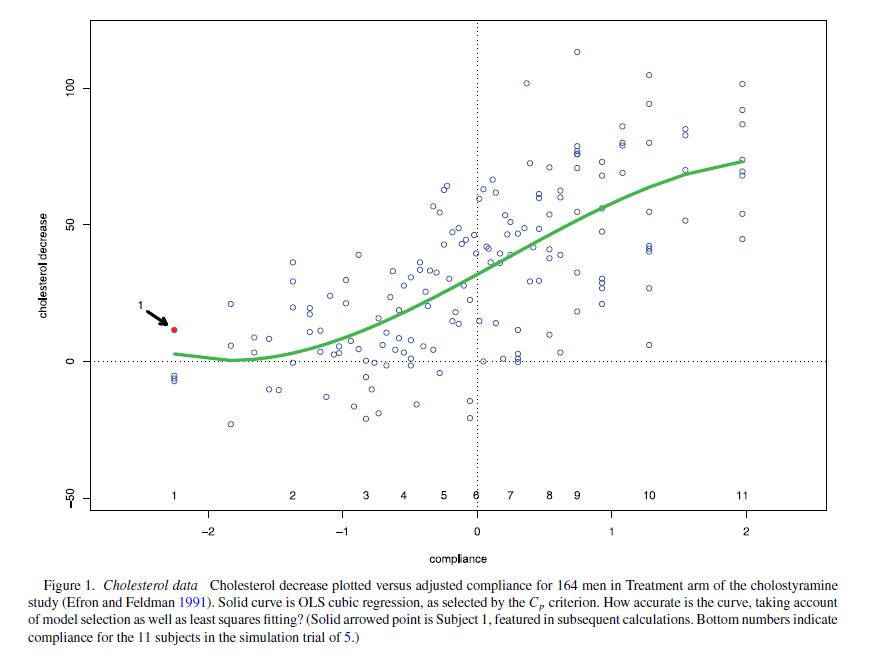
\includegraphics[width=250bp, height= 210bp]{figure1_e.png}
\end{figure}
\end{frame}
%------------------------------------------------
\begin{frame}
\frametitle{Estimation after Model Selection}
\begin{itemize}
\item My(=Bradley Efron) usual practice:\\
(a) look at data\\
(b) choose model (linear, quad, cubic $\dots$?)\\
(c) fit estimates using chosen model\\
(d) calculate standard deviation by using bootstrap\\
(e) analyze as if pre-chose
\item Question: Are we really happy with this result? 
\item My(=YC) answer: (yes..)
\end{itemize}
\end{frame}
%------------------------------------------------
\begin{frame}
\frametitle{Nonparametric bootstrap analysis}
\begin{itemize}
\item data $\mathbf{y}=\{(c_j, d_j), j=1,\dots,n=164\}= (y_1 , \dots,y_{164})$ gave original estimate
$$\hat{\mu} = X_3 \hat{\beta_3}$$
\item Bootstrap data set: $\mathbf{y^*}=(y_1 ^*, \dots,y_{164} ^*)$ where $y_j ^*$ drawn randomly and with replacement from data:
$$\rm{data} \overset{C_p} \to  m^* \overset{OLS} \to \hat{\beta}_{m^*}\to \hat{\mu} = X_{m^*} \hat{\beta}_{m^*}$$
\item Bootstrap replicates $B=4000.$
\item Then empirical standard deviation of $B$ such draws,
$$ \hat{sd}_B = \left[  \sum_{i=1} ^B  (\mu_i ^* -\mu_{\bullet} ^*)^2 \Big/ (B-1) \right] ^{1/2},$$
where $\mu_{\bullet} ^* =  \sum_{i=1} ^B \mu_i ^*/B$.
\end{itemize}
\end{frame}
%------------------------------------------------
\begin{frame}
\frametitle{$C_p$ for Cholesterol Data}
\begin{figure}[h]
\centering
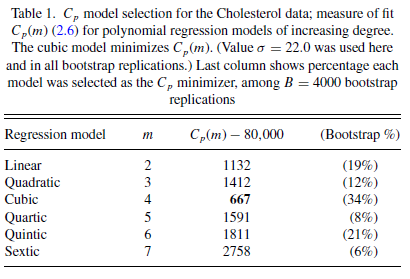
\includegraphics[width=240bp, height= 160bp]{table1_e.png}
\end{figure}
\end{frame}
%------------------------------------------------
\begin{frame}
\frametitle{Bootstrap samples}
\begin{figure}[h]
\centering
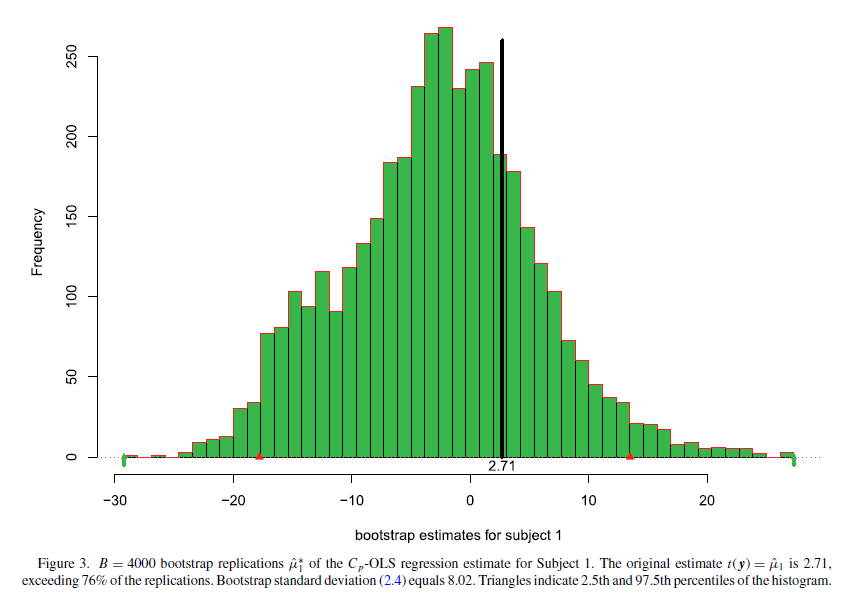
\includegraphics[width=280bp, height= 200bp]{figure3_e.png}
\end{figure}
\end{frame}
%------------------------------------------------
\begin{frame}
\frametitle{$C_p$ for Cholesterol Data}
\begin{figure}[h]
\centering
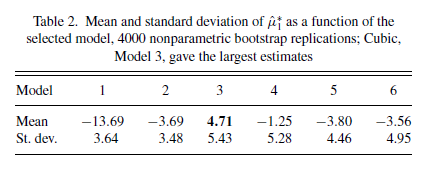
\includegraphics[width=240bp, height= 100bp]{table2_e.png}
\end{figure}
\begin{itemize}
\item The actual dataset fell into the cubic region, giving a correspondingly large estimate: model selection can make an estimate `jumpy' and erratic.
\end{itemize}
\end{frame}
%------------------------------------------------
\begin{frame}
\frametitle{Estimation after Model Selection \textbf{AGAIN}}
\begin{itemize}
\item My(=Bradley Efron) usual bad practice:\\
(a) look at data\\
(b) choose model (linear, quad, cubic $\dots$?)\\
(c) fit estimates using chosen model\\
(d) calculate confidence interval by using bootstrap\\
(e) analyze as if pre-chose
\item Question1: Are we really happy with this result? \\ 
\item Question2: How accurate is the fitted curve, taking account of the $C_p$ model-selection procedure as well as OLS estimation?
\item Answer: ??????????
\end{itemize}
\end{frame}
%------------------------------------------------
\section{Nonparametric bootstrap smoothing}
\begin{frame}
\frametitle{Estimation and Accuracy after Model Selection}
\begin{itemize}
\item Answer: Bagging (bootstrap smoothing)
\item GOAL: \\
Classical estimation theory ignored model selection out of necessity. Armed with modern computational equipment, statisticians can now deal with model-selection problems more realistically. The limited, but useful, goal of this article is to provide a general tool for the assessment of standard errors in such situations.
\end{itemize}
\end{frame}
%------------------------------------------------
\begin{frame}
\frametitle{Previous researches}
\begin{itemize}
\item Bagging (Breiman, 1996): A model-averaging device that both reduces variability and eliminates discontinuities.
\item Buja and Stuetzle (2006): An excellent recent reference.
\item Buhlmann and Yu (2002): Change hard thresholding estimators to soft thresholding.
\end{itemize}
\end{frame}
%------------------------------------------------
\begin{frame}
\frametitle{Bagging}
\begin{itemize}
\item Replace original estimator $t(\mathbf{y})$ with bootstrap average
$$\tilde{\mu} =  s(\mathbf{y}) = \sum_{i=1} ^B t(\mathbf{y_i ^*})/B$$
\item Unlike $t(\mathbf{y})$, $s(\mathbf{y})$ does not jump as $\mathbf{y}$ crosses region boundaries, making it a more dependable vehicle for setting standard errors and confidence intervals.
\end{itemize}
\end{frame}
%------------------------------------------------
\begin{frame}
\frametitle{Bootstrap confidence intervals}
\begin{itemize}
\item Standard: $\hat{\mu} \pm 1.96 \hat{sd}_B$
\item Percentile: $[\hat{\mu}^{*(.025)},\hat{\mu}^{*(.975)}]$
\item Smoothed Standard: $\tilde{\mu} \pm 1.96 \tilde{sd}_B$ \\
where $\tilde{sd}_B$ is a standard deviation for the smoothed bootstrap estimate $\tilde{\mu}$
\end{itemize}
\end{frame}
%------------------
\begin{frame}
\frametitle{Bootstrap confidence intervals}
\begin{itemize}
\item A brute force approach employs a second level of bootstrapping: resampling $y_i ^*$ yields a collection of $B$ second-level replications $y_{ij} ^{**}$ from which we calculate $s_i ^* = \sum t(y_{ij} ^{**}) / B$
\item Requires an enormous number of recomputations of the original statistics $t(\cdot)$.
\end{itemize}
\end{frame}
%------------------
\section{Take a break}
\begin{frame}
\frametitle{Duplicate the paper}
\begin{figure}[h]
\centering
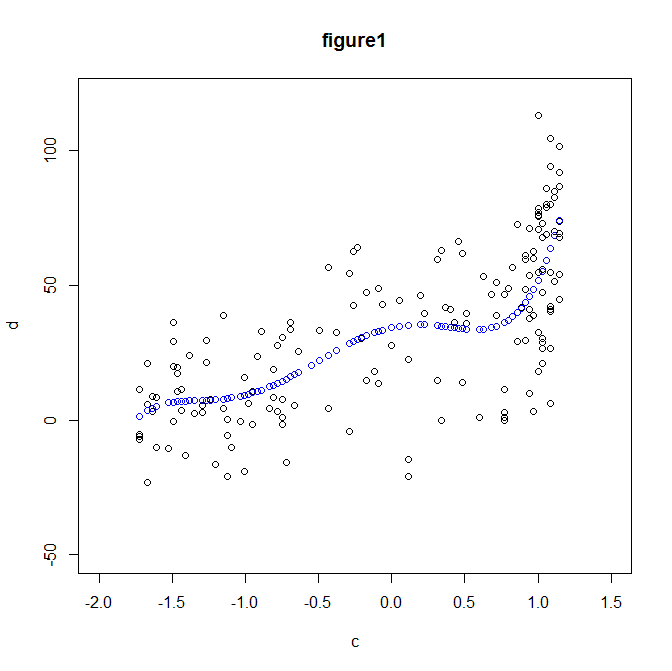
\includegraphics[width=200bp, height= 180bp]{figure1.png}
\caption{Cholesterol data, n=164 subjects: cholesterol decrease plotted versus normalized compliance; Blue points indicate OLS fifth degree polynomial regression}
\end{figure}
\end{frame}
%------------------------------------------------
\begin{frame}
\frametitle{Duplicate the paper}
\begin{table}[]
\centering
\caption{$\sigma=22.0$ from ``full model''}
\label{my-label}
\begin{tabular}{lllll}
\hline
{Model}   & {df} & {$C_p-80000$} & {(Boot \%)}\\ \hline
linear           & 2           & 1105                 & 2.8                        \\
quad             & 3           & 233                  & 3.3                       \\
cubic            & 4           & -54                  & 2.8                      \\
quadratic        & 5           & -2335                & 15.5          \\
\textbf{quintic} & \textbf{6}  & \textbf{-3058}       & \textbf{43.6}                 \\
sextic           & 7           & -2744                & 31.6                \\ \hline
\end{tabular}
\end{table}
\end{frame}
%------------------------------------------------
\begin{frame}
\frametitle{Duplicate the paper}
\begin{figure}[h]
\centering
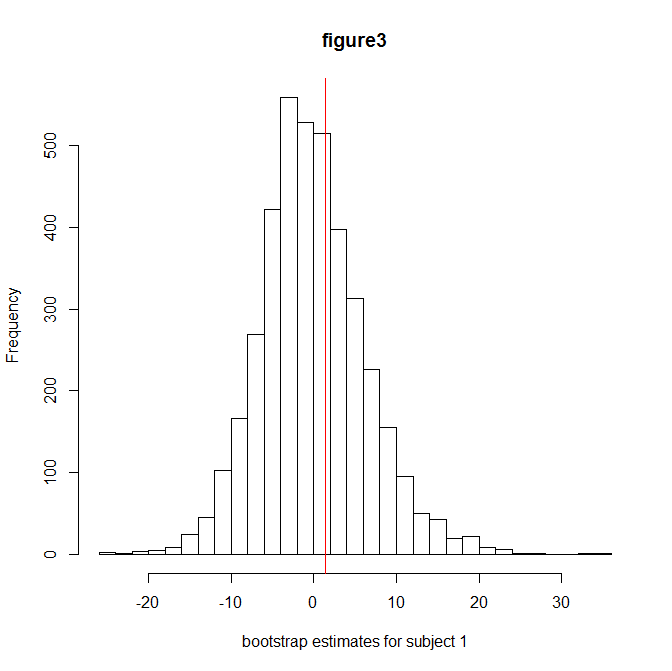
\includegraphics[width=200bp, height= 180bp]{figure3.png}
\caption{B=4000 nonparametric bootstrap replications for the model-selected regression estimate of Subject 1; 63.2\% of the replications less than original estimate}
\end{figure}
\end{frame}
%------------------------------------------------
\begin{frame}
\frametitle{Duplicate the paper}
\begin{table}[]
\centering
\caption{Mean and standard deviation of $\hat{\mu}_1 ^*$ as a function of the selected model, 4000 nonparametric bootstrap replications}
\label{my-label}
\begin{tabular}{|l|l|l|l|l|l|l|}
\hline
\textbf{Model} & \textbf{1} & \textbf{2} & \textbf{3} & \textbf{4} & \textbf{5}     & \textbf{6} \\ \hline
\textbf{Mean}  & -1.34      & 5.04       & -1.34      & 8.71       & \textbf{-0.08} & -4.81      \\ \hline
\textbf{Std}   & 2.60       & 2.92       & 3.55       & 5.58       & \textbf{4.52}  & 4.78       \\ \hline
\end{tabular}
\end{table}
\end{frame}
%------------------------------------------------
\section{Accuracy of the smoothed bootstrap estimates}
\begin{frame}
\frametitle{Notations}
\begin{itemize}
\item $s_0 = s(\mathbf{y}), t_i ^* = t( \mathbf{y_i ^*})$
\item $Y_{ij} ^* = \#\{y_{ik} ^* = y_{j} \}$ : the number of elements of $\mathbf{y_i ^*}$ equaling the original data point $y_j$.
\item The vector $Y_i ^* = (Y_{i1} ^*, \dots, Y_{in} ^*)$ follows a multinomial distribution with $n$ draws on $n$ categories each of probability $1/n$, and has mean vector and covariance matrix 
$$Y_i ^* \sim (\mathbf{1_n}, I_n \mathbf{- 1_n 1_n ^{'}} /n) $$
\end{itemize}
\end{frame}
%------------------------------------------------
\begin{frame}
\frametitle{Accuracy Theorem}
\begin{theorem}
The nonparametric delta-method estimate of standard deviation for the ideal smoothed bootstrap statistic $s(\mathbf{y}) = \sum_{i=1} ^B t(\mathbf{y_i ^*}) /B$ is
$$ \tilde{sd} = \left[ \sum_{j=1} ^N cov_j ^2\right] ^{1/2}$$
where
$$ cov_j = cov_* (Y_{ij} ^* , t_i ^*),$$
the bootstrap covariance between $Y_{ij} ^*$ and $t_i ^*$.
\end{theorem}
\end{frame}
%------------------------------------------------
\begin{frame}
\frametitle{Accuracy Theorem}
\begin{figure}[h]
\centering
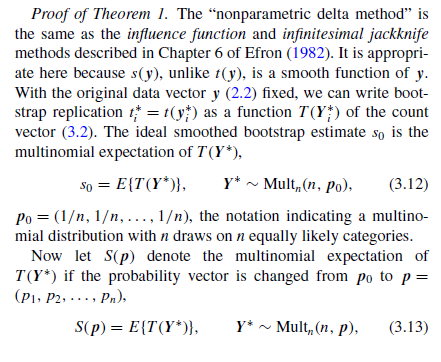
\includegraphics[width=220bp, height= 180bp]{proof1_e.png}
\end{figure}
\end{frame}
%------------------------------------------------
\begin{frame}
\frametitle{Accuracy Theorem}
\begin{figure}[h]
\centering
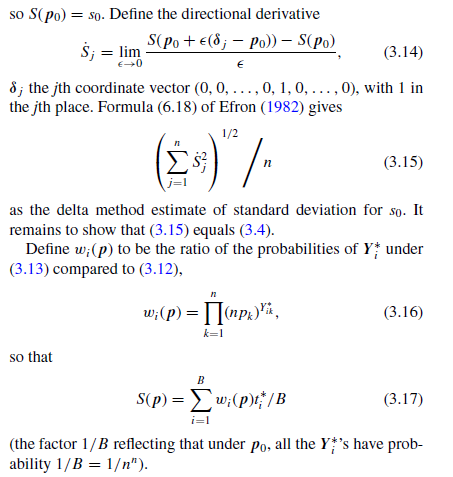
\includegraphics[width=220bp, height= 180bp]{proof2_e.png}
\end{figure}
\end{frame}
%------------------------------------------------
\begin{frame}
\frametitle{Accuracy Theorem}
\begin{figure}[h]
\centering
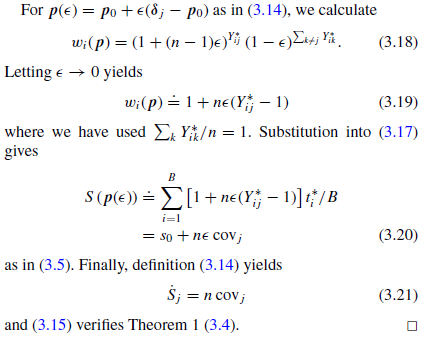
\includegraphics[width=220bp, height= 180bp]{proof3_e.png}
\end{figure}
\end{frame}
%------------------------------------------------
\begin{frame}
\frametitle{Sample version of Accuracy Theorem}
\begin{itemize}
\item The estimate of standard deviation in the non-ideal case is similar: $$ \tilde{sd} = \left[ \sum_{j=1} ^N \widehat{cov}_j ^2\right] ^{1/2}$$
where
$$ \widehat{cov}_j = \sum_{i=1} ^B (Y_{ij} ^* - Y_{\bullet j} ^*) (t_i ^* - t_{\bullet} ^*) /B$$
with $Y_{\bullet j} ^* = \sum_{i=1} ^B Y_{ij} ^* /B$ and $t_{\bullet} ^* = \sum_{i=1} ^B t_{i} ^* /B$
\item Note that
$$ \hat{sd}_B = \left[ \sum_{i=1} ^B (t_i^* - t_{\bullet} ^*) ^2\right] ^{1/2}$$
\end{itemize}
\end{frame}
%------------------------------------------------
\begin{frame}
\frametitle{Sample version of Accuracy Theorem}
\begin{itemize}
\item Let $\mathcal{L}(Y^*)$ be the (n-1) dimensional subspace of $\mathcal{R}^B$ spanned by the columns of the $B \times n$ matrix having elements $Y_{ij} ^* -1 $.
\item Also define $$ U^* = \mathbf{t} - s_o \mathbf{1}.$$
Note that $U^*$ is the $B$-vector of mean-centered replications $t_i^* - s_0$.
\end{itemize}
\end{frame}
%------------------------------------------------
\begin{frame}
\frametitle{Accuracy Theorem}
\begin{corollary}
The ratio $\tilde{sd}_B / \hat{sd}_B$ is given by
$$ \frac{\tilde{sd}_B}{\hat{sd}_B} = \frac{\| \hat{U}^* \|}{\| U^* \|}$$
where $\hat{U}^* $ is the projection of $U^* $ into $\mathcal{L}(Y^*)$.
\end{corollary}
\end{frame}
%------------------------------------------------
\begin{frame}
\frametitle{Accuracy Theorem}
\begin{figure}[h]
\centering
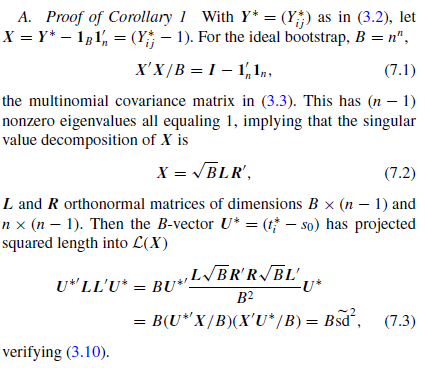
\includegraphics[width=200bp, height= 190bp]{proof4_e.png}
\end{figure}
\end{frame}
%------------------------------------------------
\begin{frame}
\frametitle{Accuracy Theorem}
\begin{figure}[h]
\centering
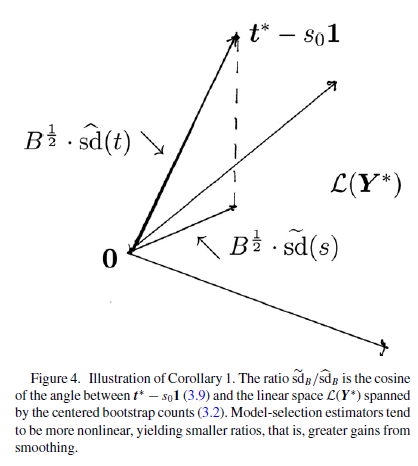
\includegraphics[width=180bp, height= 220bp]{figure4_e.png}
\end{figure}
\end{frame}
%------------------------------------------------
\begin{frame}
\frametitle{Accuracy Theorem}
\begin{figure}[h]
\centering
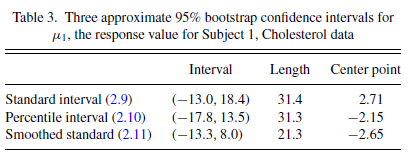
\includegraphics[width=220bp, height= 90bp]{table3_e.png}
\end{figure}
\end{frame}
%------------------------------------------------
\begin{frame}
\frametitle{Accuracy Theorem}
\begin{table}[]
\centering
\caption{Three approximate 95\% bootstrap confidence intervals for $\mu_1$, the response value for Subject 1, Cholesterol data}
\label{my-label}
\begin{tabular}{rrrrrrrrrrr}
\hline
& Left & Right & Center point\\
\hline
Standard interval &  -11.270996 &14.135120 & 1.432062\\
Percentile interval & -11.822923 &14.223378 & 1.200228\\
Smoothed standard & -9.445251 & 9.219275 & -0.112988\\
\hline
\end{tabular}
\end{table}
\end{frame}
%------------------------------------------------
\begin{frame}
\frametitle{Accuracy Theorem}
\begin{figure}[h]
\centering
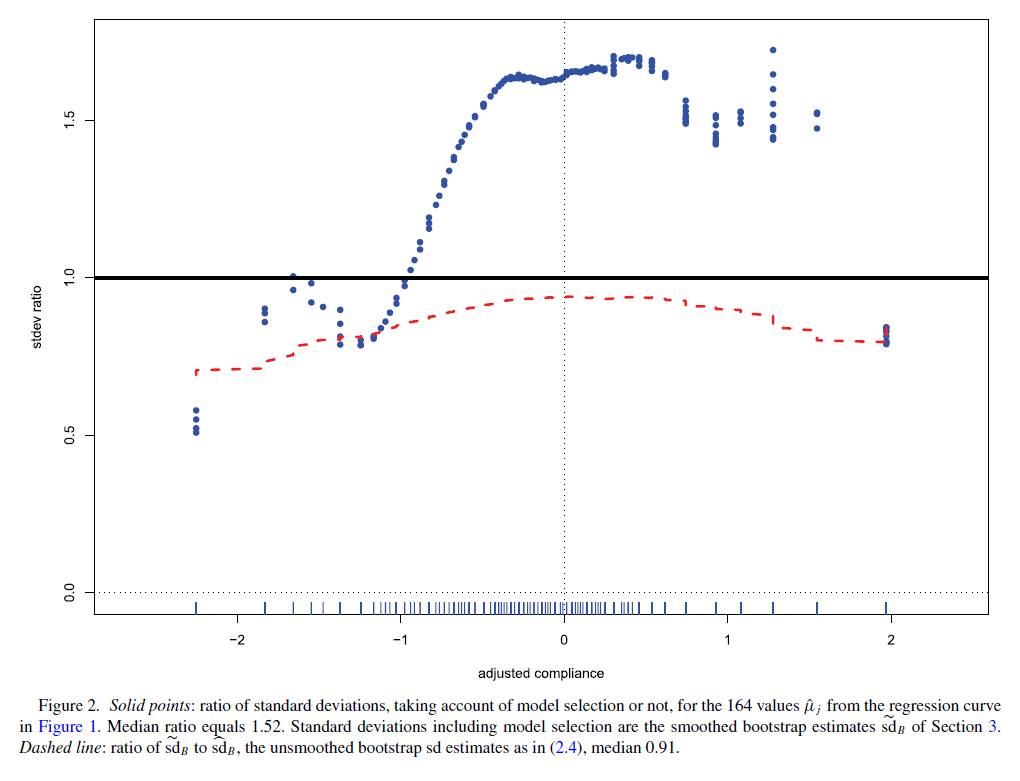
\includegraphics[width=270bp, height= 200bp]{figure2_e.png}
\end{figure}
\end{frame}
%------------------------------------------------
\begin{frame}
\frametitle{How many bootstrap replications $B$ are necessary?}
\begin{itemize}
\item The jackknife provides a quick answer: divide the $B$ replications into $J$ groups of size $B/J$ each, and let $\tilde{sd}_{B j}$ be the estimate for $\tilde{sd}_{B}$ computed with the $j$th group removed.
$$ \tilde{cv}_B = \left[ \frac{J}{J-1} \sum_{j=1} ^J ( \tilde{sd}_{B j}- \tilde{sd}_{B \bullet})^2 \right]^{1/2} \Big/ \tilde{sd}_B $$
where $ \tilde{sd}_{B \bullet} = \sum \tilde{sd}_{B j}/J$, is the jackknife estimated coefficient of variation for $\tilde{sd}_B$.
\item  For $B= 4000$ , $ \tilde{cv}_B = 0.02$ and it would have been quite sufficient.
\end{itemize}
\end{frame}
%------------------------------------------------
\section{Parametric bootstrap smoothing}
\begin{frame}
\frametitle{Background}
\begin{itemize}
\item Assume $$f_\alpha(\hat{\beta}) = e^{\alpha'\hat{\beta} - \psi(\alpha)} f_0(\hat{\beta})$$
where $\alpha$ is the $p$-dimensional canonical parameter vector, $\hat{\beta}$ the $p$-dimensional sufficient statistic vector (playing the role of $\mathbf{y}$ ), $\psi(\alpha)$ the cumulant generating function, and $f_0(\hat{\beta})$ the ``carrying density''.
\item Under mild conditions, the expectation parameter $\beta= E_\alpha (\hat{\beta})$ is a one-to-one function of $\alpha$, say $\beta = \lambda(\alpha)$, having $p\times p$ derivative matrix
$$ \frac{d\beta}{d\alpha} = V(\alpha),$$
where $V$ is the covariance matrix. 
\item Then the maximum likelihood estimate (MLE) of $\alpha$ is obtained by $\lambda^{-1}(\hat{\beta})$.
\end{itemize}
\end{frame}
%------------------------------------------------
\begin{frame}
\frametitle{Parametric bootstrap}
\begin{itemize}
\item A parametric bootstrap sample is obtained by drawing iid realizations $\hat{\beta}^*$ from the MLE density $f_{\hat{\alpha}}(\cdot)$.
\item If $\hat{\mu} = t(\hat{\beta})$ is an estimate of a parameter interest $\mu$, we have a smoothed estimate,
$$ \tilde{\mu} = \sum_{i=1} ^B t(\hat{\beta}_i ^*)/B.$$
\item When $t(\cdot)$ involves model selection, $\hat{\mu}$ is liable to an erratic, jumpiness, smoothed out by the averaging process.
\end{itemize}
\end{frame}
%------------------------------------------------
\begin{frame}
\frametitle{Parametric bootstrap}
\begin{itemize}
\item Let $\mathbb{B}$ be the $B \times p$ matrix with $i$th row $\hat{\beta}_i ^*-\hat{\beta}$. Then
$$ \mathbb{B}^{'} \mathbf{1_B}/B = \mathbb{O}, \qquad \mathbb{B}^{'} \mathbb{B} = \hat{V}.$$
\item As the procedure for nonparametric bootstrap, 
$$ cov_* = \mathbb{B}^{'} (\mathbf{t^*} - s_0 \mathbf{1_B})/B $$
\end{itemize}
\end{frame}
%------------------------------------------------
\begin{frame}
\frametitle{Accuracy theorem for parametric version}
\begin{theorem}
The parametric delta-method estimate of standard deviation for the ideal smoothed estimate is
$$\tilde{sd} = [cov_* ^{`} \hat{V} ^{-1} cov_*]^{1/2}$$
\end{theorem}
\begin{corollary}
For $$ \hat{sd} = [ \| (\mathbf{t^*} - s_0 \mathbf{1_B}) \| ^2 /B ]^{1/2},$$
the ratio $\tilde{sd} / \hat{sd}$ is given by
$$ B^{1/2}[ (\mathbf{t^*} - s_0 \mathbf{1_B})^{`} \mathbb{B} (\mathbb{B}^{'}\mathbb{B})^{-1} \mathbb{B}^{'} (\mathbf{t^*} - s_0 \mathbf{1_B}) ]^{1/2}/ \hat{sd}$$
\end{corollary}
\end{frame}
%------------------------------------------------
\begin{frame}
\frametitle{Schematic diagram of estimation without model selection}
\begin{figure}[h]
\centering
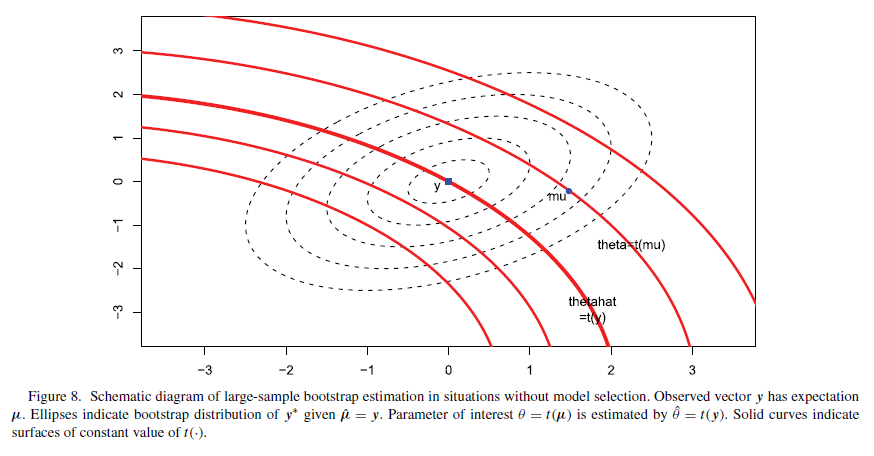
\includegraphics[width=320bp, height= 200bp]{figure8_e.png}
\end{figure}
\end{frame}
%------------------------------------------------
\begin{frame}
\frametitle{Estimation after model selection}
\begin{figure}[h]
\centering
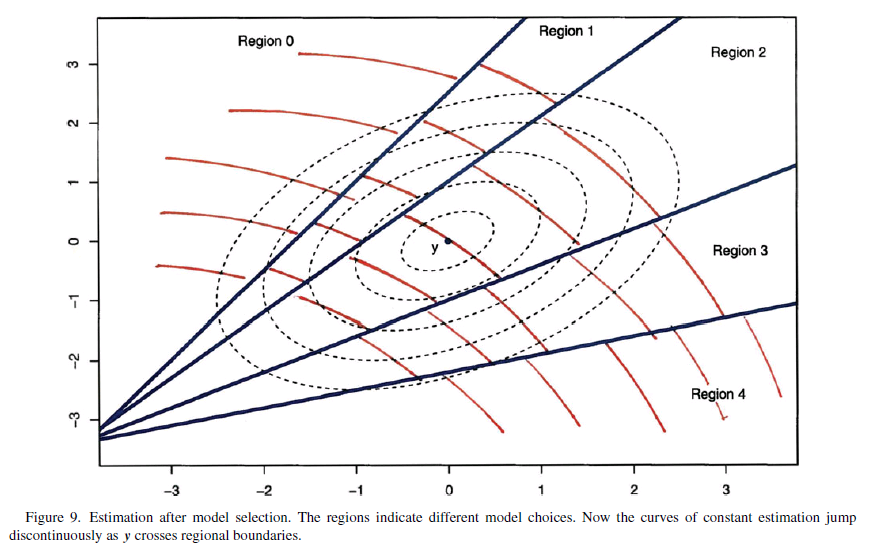
\includegraphics[width=300bp, height= 200bp]{figure9_e.png}
\end{figure}
\end{frame}
%------------------------------------------------
\section{Discussions}
\begin{frame}
\frametitle{What we covered}
\begin{itemize}
\item Bootstrap!
\end{itemize}
\end{frame}
%------------------
\begin{frame}
\frametitle{What we didn't cover or questions}
\begin{itemize}
\item Discrete random variable (or repeated random variable)
\item Better bootstrap confidence intervals
\item Asymptotic performance
\item Real data problems
\end{itemize}
\end{frame}
%------------------
\end{document}








